\documentclass {article}
\usepackage[margin=1 in]{geometry}
\usepackage{graphicx}

\begin{document}

\section{Uncalibrated CPU and GPU images: LBA\_OUTER}

\begin{figure*}
\center{
 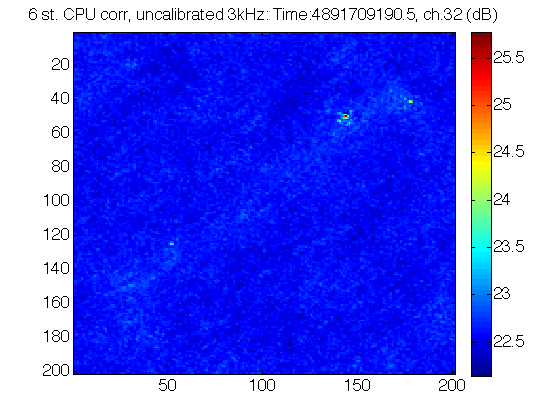
\includegraphics [width=0.6\columnwidth]{Figs/uncal_cpu_ch32_6station.png}
 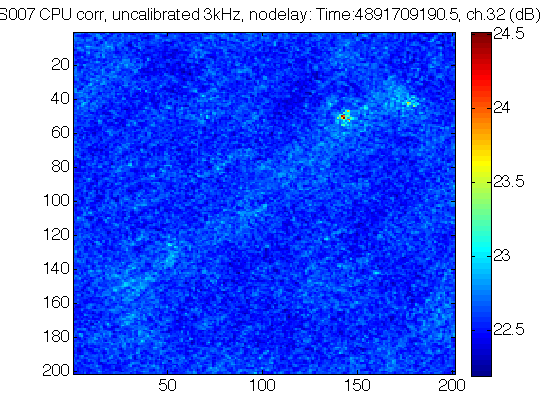
\includegraphics [width=0.6\columnwidth]{Figs/uncal_cpu_ch32_6station_nodelay.png}
 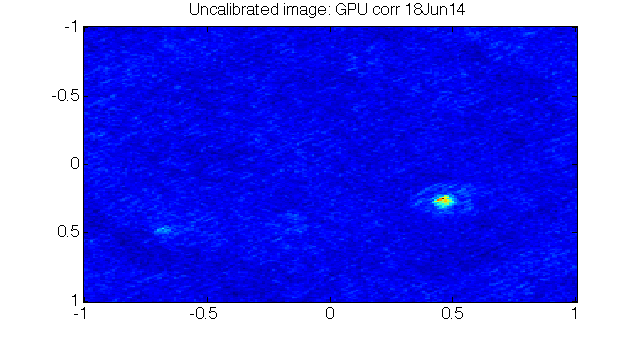
\includegraphics [width=0.6\columnwidth]{Figs/gpucorr_uncalmap.png}
 \caption {Uncalibrated 6station images. CPU correlated with inter station delays (top), without interstation delays applied (mid). 3kHz/1sec on 21-Nov-2013 00:06:30. (Bottom) GPU correlated uncalibrated image (3kHz/1sec) on 18 Jul 14shows the Sun.} 
}
\end{figure*}

\begin{figure*}
\center{
 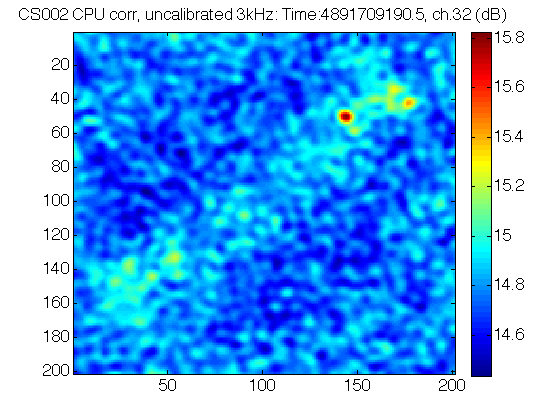
\includegraphics [width=0.45\columnwidth]{Figs/uncal_cpu_ch32_cs002.png}
 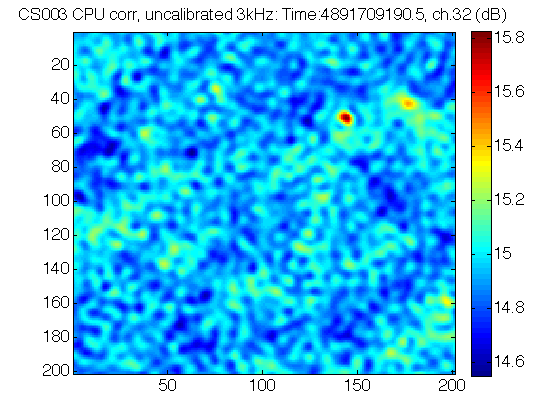
\includegraphics [width=0.45\columnwidth]{Figs/uncal_cpu_ch32_cs003.png}
 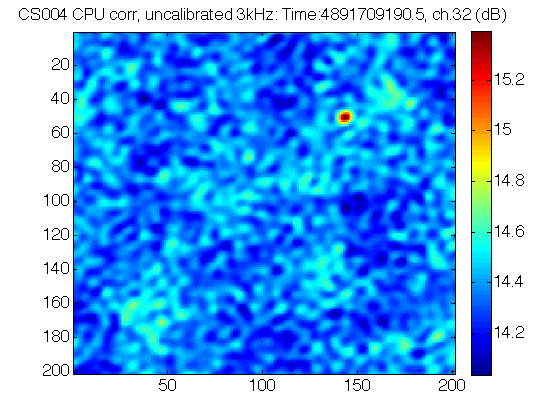
\includegraphics [width=0.45\columnwidth]{Figs/uncal_cpu_ch32_cs004.png}
 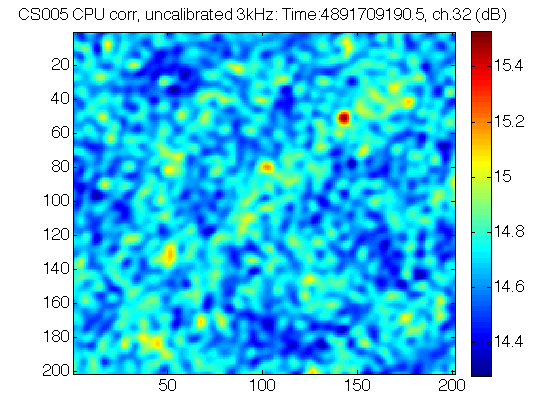
\includegraphics [width=0.45\columnwidth]{Figs/uncal_cpu_ch32_cs005.png}
 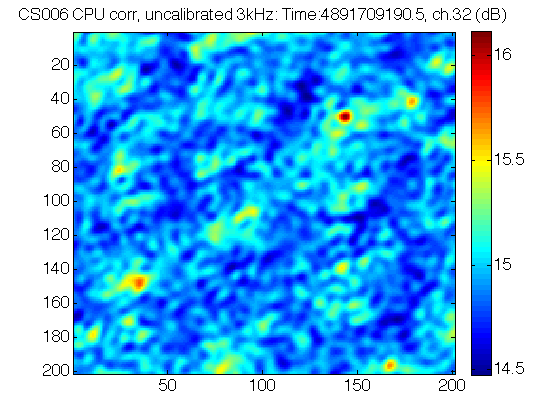
\includegraphics [width=0.45\columnwidth]{Figs/uncal_cpu_ch32_cs006.png}
 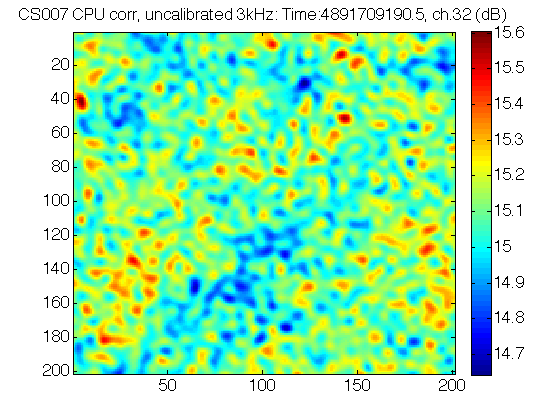
\includegraphics [width=0.45\columnwidth]{Figs/uncal_cpu_ch32_cs007.png}
 \caption {Uncalibrated individual station images, CPU correlated. 3kHz/1sec on 21-Nov-2013 00:06:30} 
}
\end{figure*}

\begin{figure*}
\center{
 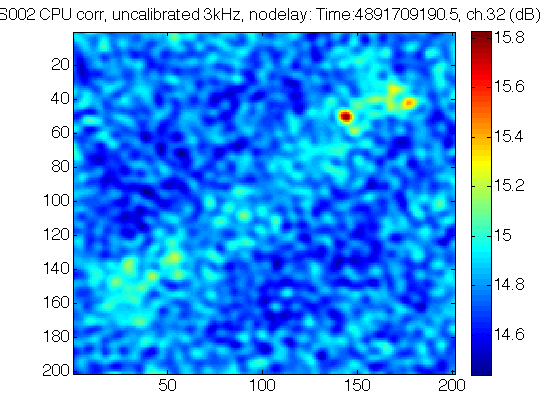
\includegraphics [width=0.45\columnwidth]{Figs/uncal_cpu_ch32_cs002_nodelay.png}
 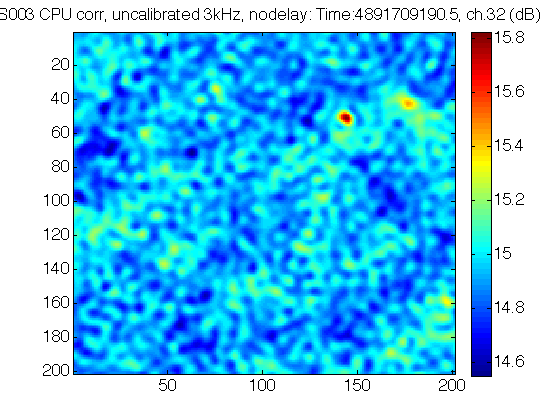
\includegraphics [width=0.45\columnwidth]{Figs/uncal_cpu_ch32_cs003_nodelay.png}
 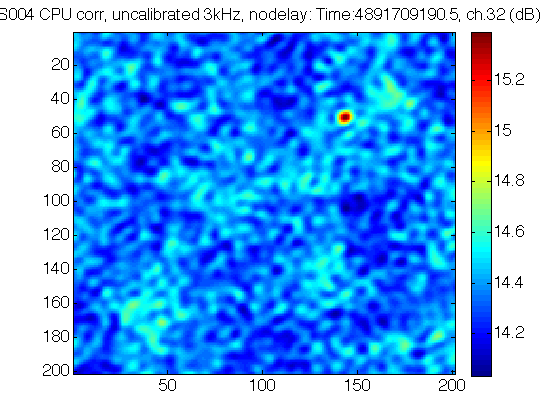
\includegraphics [width=0.45\columnwidth]{Figs/uncal_cpu_ch32_cs004_nodelay.png}
 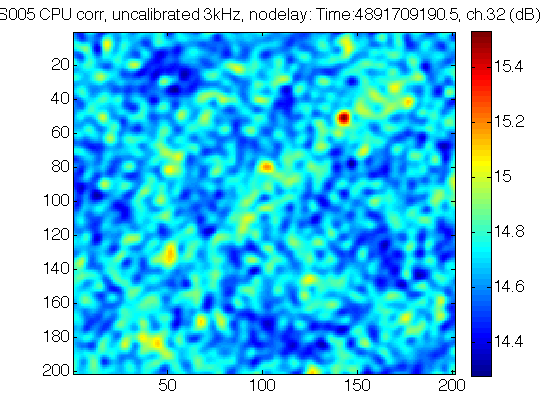
\includegraphics [width=0.45\columnwidth]{Figs/uncal_cpu_ch32_cs005_nodelay.png}
 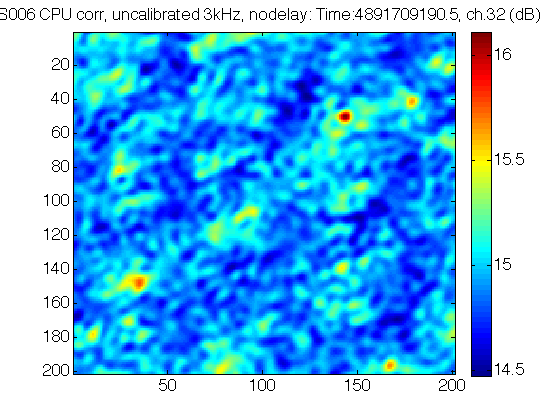
\includegraphics [width=0.45\columnwidth]{Figs/uncal_cpu_ch32_cs006_nodelay.png}
 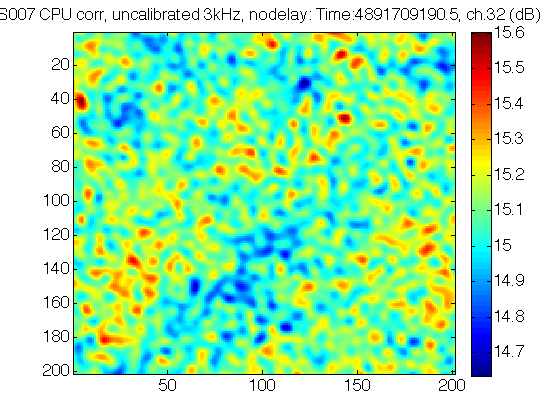
\includegraphics [width=0.45\columnwidth]{Figs/uncal_cpu_ch32_cs007_nodelay.png}
 \caption {Uncalibrated individual station images, CPU correlated.No inter-station delays applied. 3kHz/1sec on 21-Nov-2013 00:06:31} 
}
\end{figure*}

\section{3-station images: GPU}
Live raw SDO data was recorded from 3 stations (CS00[3,5,7]) using the udp-copy-stations.sh script. These were correlated using the run.off.del and run.off.nodel (off=offline, del=delay applied) scripts. A single channel (No. 32) was  extracted using the rdgpuvis.c program and imaged in matlab using the gengpusubarrayimag.m script.

\begin{figure*}
\center{
 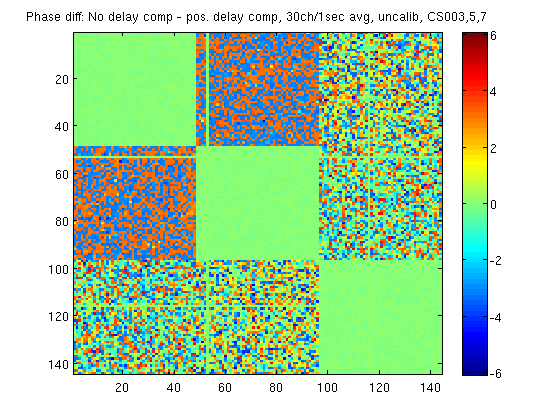
\includegraphics [width=0.45\columnwidth]{Figs/uncal_gpu_ch20-50_cs3_5_7_acc_phdiff_nodel_pos.png}
 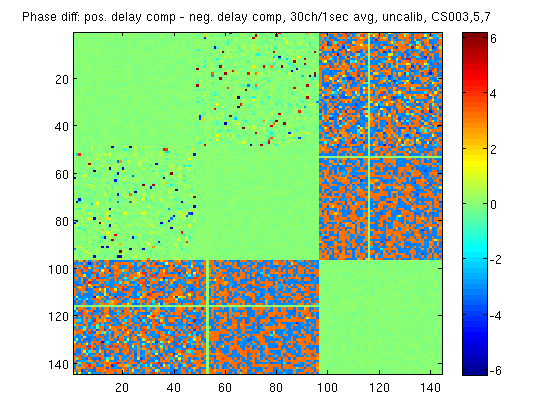
\includegraphics [width=0.45\columnwidth]{Figs/uncal_gpu_ch20-50_cs3_5_7_acc_phdiff_pos_neg.png}
 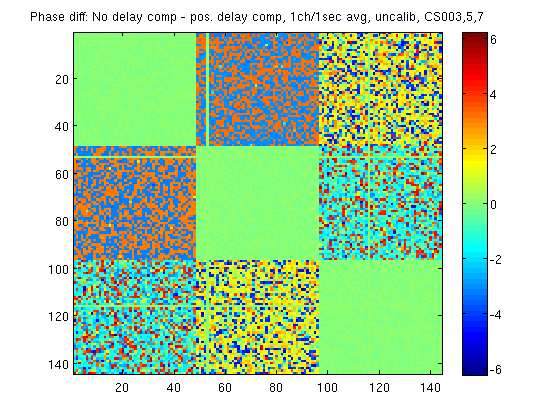
\includegraphics [width=0.45\columnwidth]{Figs/uncal_gpu_ch31-32_cs3_5_7_acc_phdiff_nodel_pos.png}
 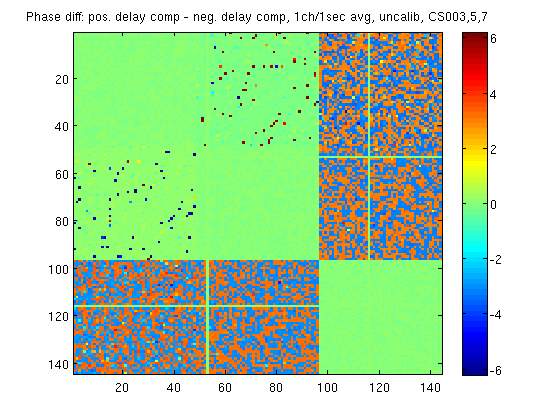
\includegraphics [width=0.45\columnwidth]{Figs/uncal_gpu_ch31-32_cs3_5_7_acc_phdiff_pos_neg.png}
 \caption {Uncalibrated 3station phase difference, GPU correlated. 30ch/1sec avg (top) and 1ch/1sec avg (bottom). No delay compensation - pos. delay compensation. (left), pos. delay compensation - neg. delay compensation (right).} 
}
\end{figure*}

\begin{figure*}
\center{
 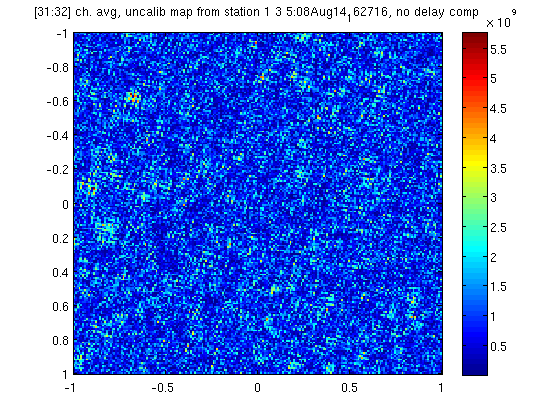
\includegraphics [width=0.45\columnwidth]{Figs/uncal_gpu_ch31-32_cs3_5_7_nodel.png}
 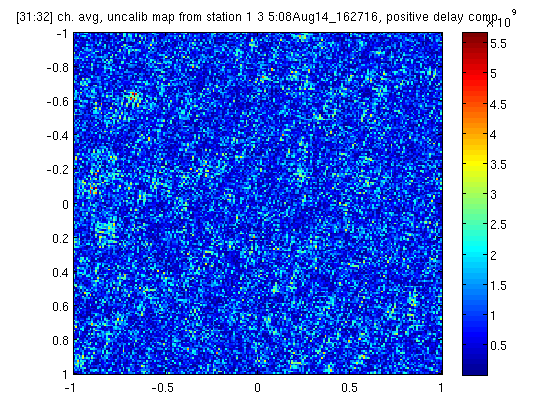
\includegraphics [width=0.45\columnwidth]{Figs/uncal_gpu_ch31-32_cs3_5_7_posdel.png}
 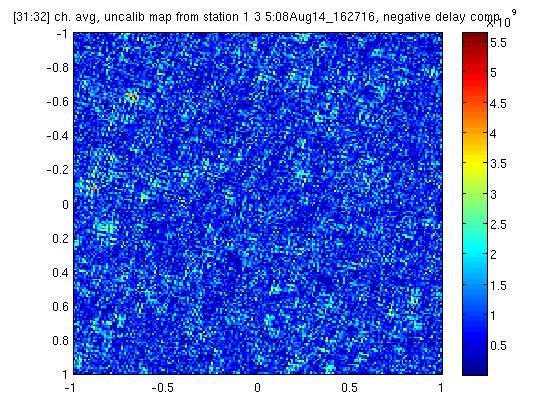
\includegraphics [width=0.45\columnwidth]{Figs/uncal_gpu_ch31-32_cs3_5_7_negdel.png}
 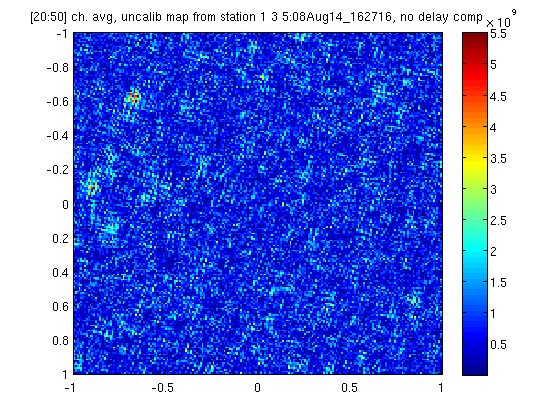
\includegraphics [width=0.45\columnwidth]{Figs/uncal_gpu_ch20-50_cs3_5_7_nodel.png}
 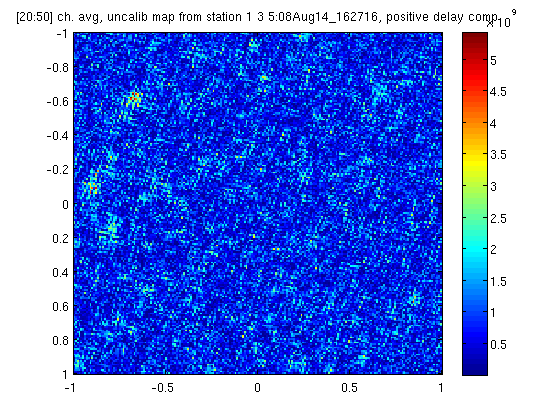
\includegraphics [width=0.45\columnwidth]{Figs/uncal_gpu_ch20-50_cs3_5_7_posdel.png}
 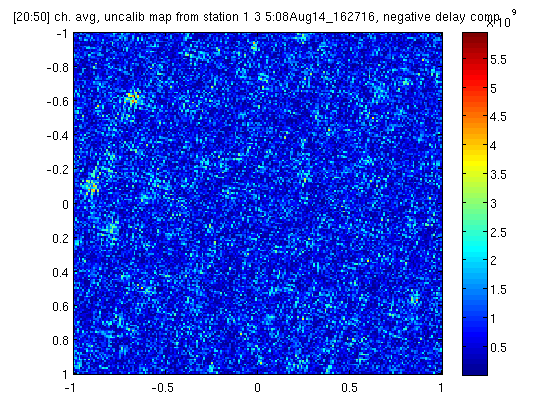
\includegraphics [width=0.45\columnwidth]{Figs/uncal_gpu_ch20-50_cs3_5_7_negdel.png}
 \caption {Uncalibrated 3station images, GPU correlated. 30ch/1sec avg (top).} 
}
\end{figure*}

\section{3-station images: CPU}
\begin{figure*}
\center{
 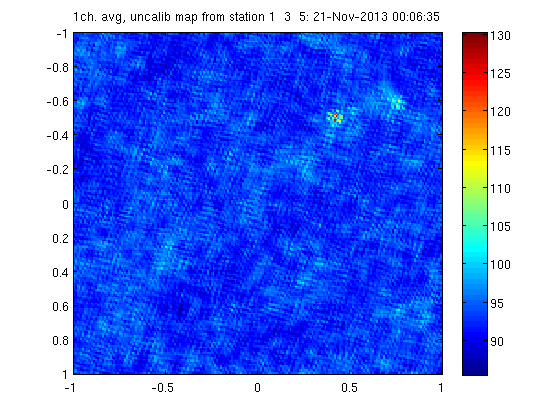
\includegraphics [width=0.45\columnwidth]{Figs/uncal_cpu_ch31-32_cs3_5_7_del.png}
 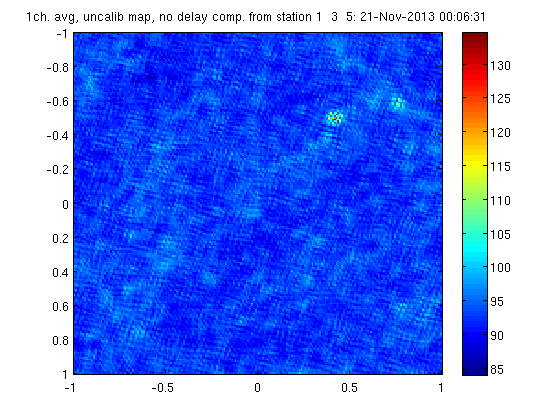
\includegraphics [width=0.45\columnwidth]{Figs/uncal_cpu_ch31-32_cs3_5_7_nodel.png}
 \caption {Uncalibrated 3station images, CPU correlated. 1ch/1sec avg, with delay compensation (top), without delay compensation (bottom).} 
}
\end{figure*}

\end{document}
